\begin{equation}
\langle \widetilde{\delta} ({\bf k}) \widetilde{\delta} ({\bf k'}) \rangle = (2 \pi) ^3 \delta_D \left( {\bf k} - {\bf k'} \right) P \left({\bf k} \right)
\end{equation}

We can estimate the power spectrum with the relational

\begin{equation}
P\left( k\right) \approx \frac{\sum_{\textbf{k} \in k}\langle | \widetilde{\delta} \left( \textbf{k}\right) |^2 \rangle}{N_k V}
\end{equation}

\begin{equation}
    \widetilde{\Delta}^2 \left( k \right) = \frac{k^3}{2 \pi ^2} P \left( k \right)
\end{equation}

\begin{align}
    &\Delta^2_{\textrm{Ly} \alpha} \left( k \right) = \left( \nu \bar{I}_{\nu} \right)^2 \widetilde{\Delta}^2_{\textrm{Ly} \alpha} \left( k \right) \\
    &\Delta^2_{21}\left( k \right) = \left(\delta \overline{T}_b \right)^2 \widetilde{\Delta}^2_{21} \left( k \right) \\
    &\Delta^2_{21, \textrm{Ly} \alpha} \left( k \right) = \left(\delta \overline{T}_b \right) \left( \nu \bar{I}_{\nu} \right) \widetilde{\Delta}^2_{21, \textrm{Ly} \alpha} \left( k \right)
\end{align}

\begin{equation}
  r \left(k \right) = \frac{\Delta^2_{21, \textrm{Ly} \alpha}\left(k \right)}
                           {\sqrt{\Delta^2_{21} \left(k \right)\Delta^2_{\textrm{Ly} \alpha} \left(k \right)}}
\end{equation}

\begin{figure}[ht]
	\centering
	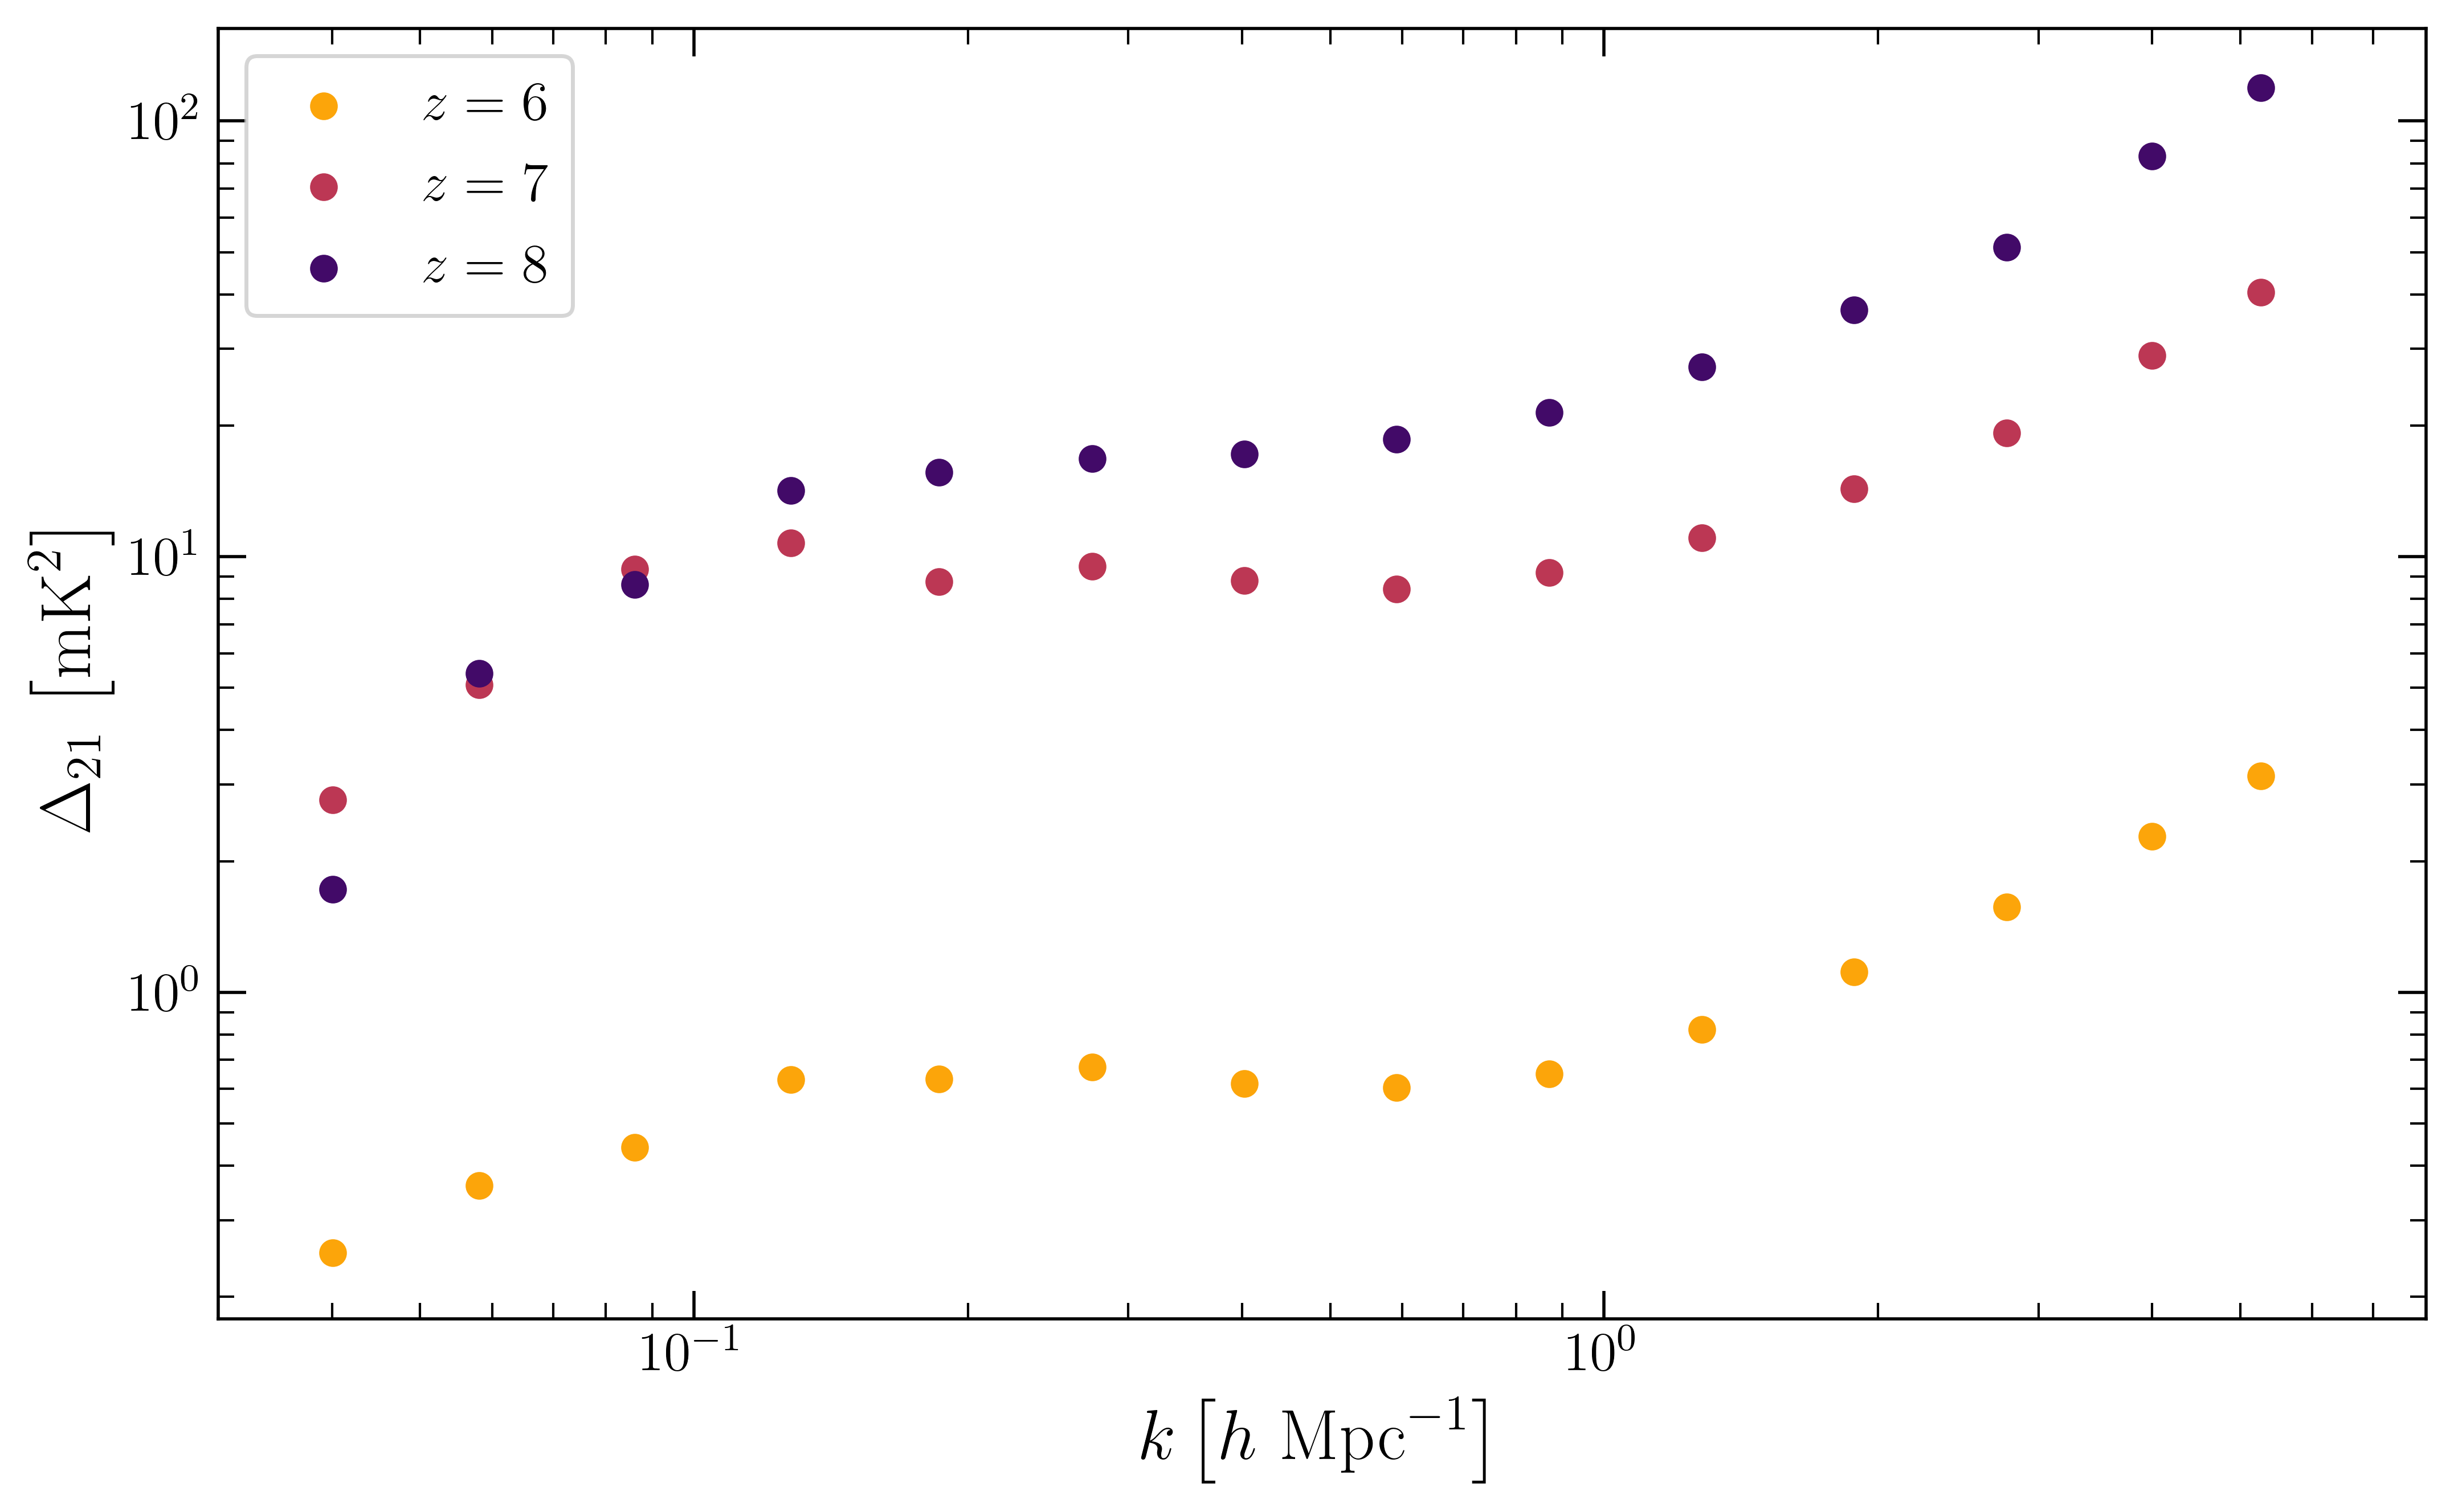
\includegraphics[width=1.\textwidth]{21cm_power_spectrum.png}
	\caption[21\,cm Power Spectrum]{21\,cm power spectra plotted as a function of redshift for the fiducial \fastsim\
           model.}
	\label{fig:21cm_ps}
\end{figure}

\begin{figure}[ht]
	\centering
	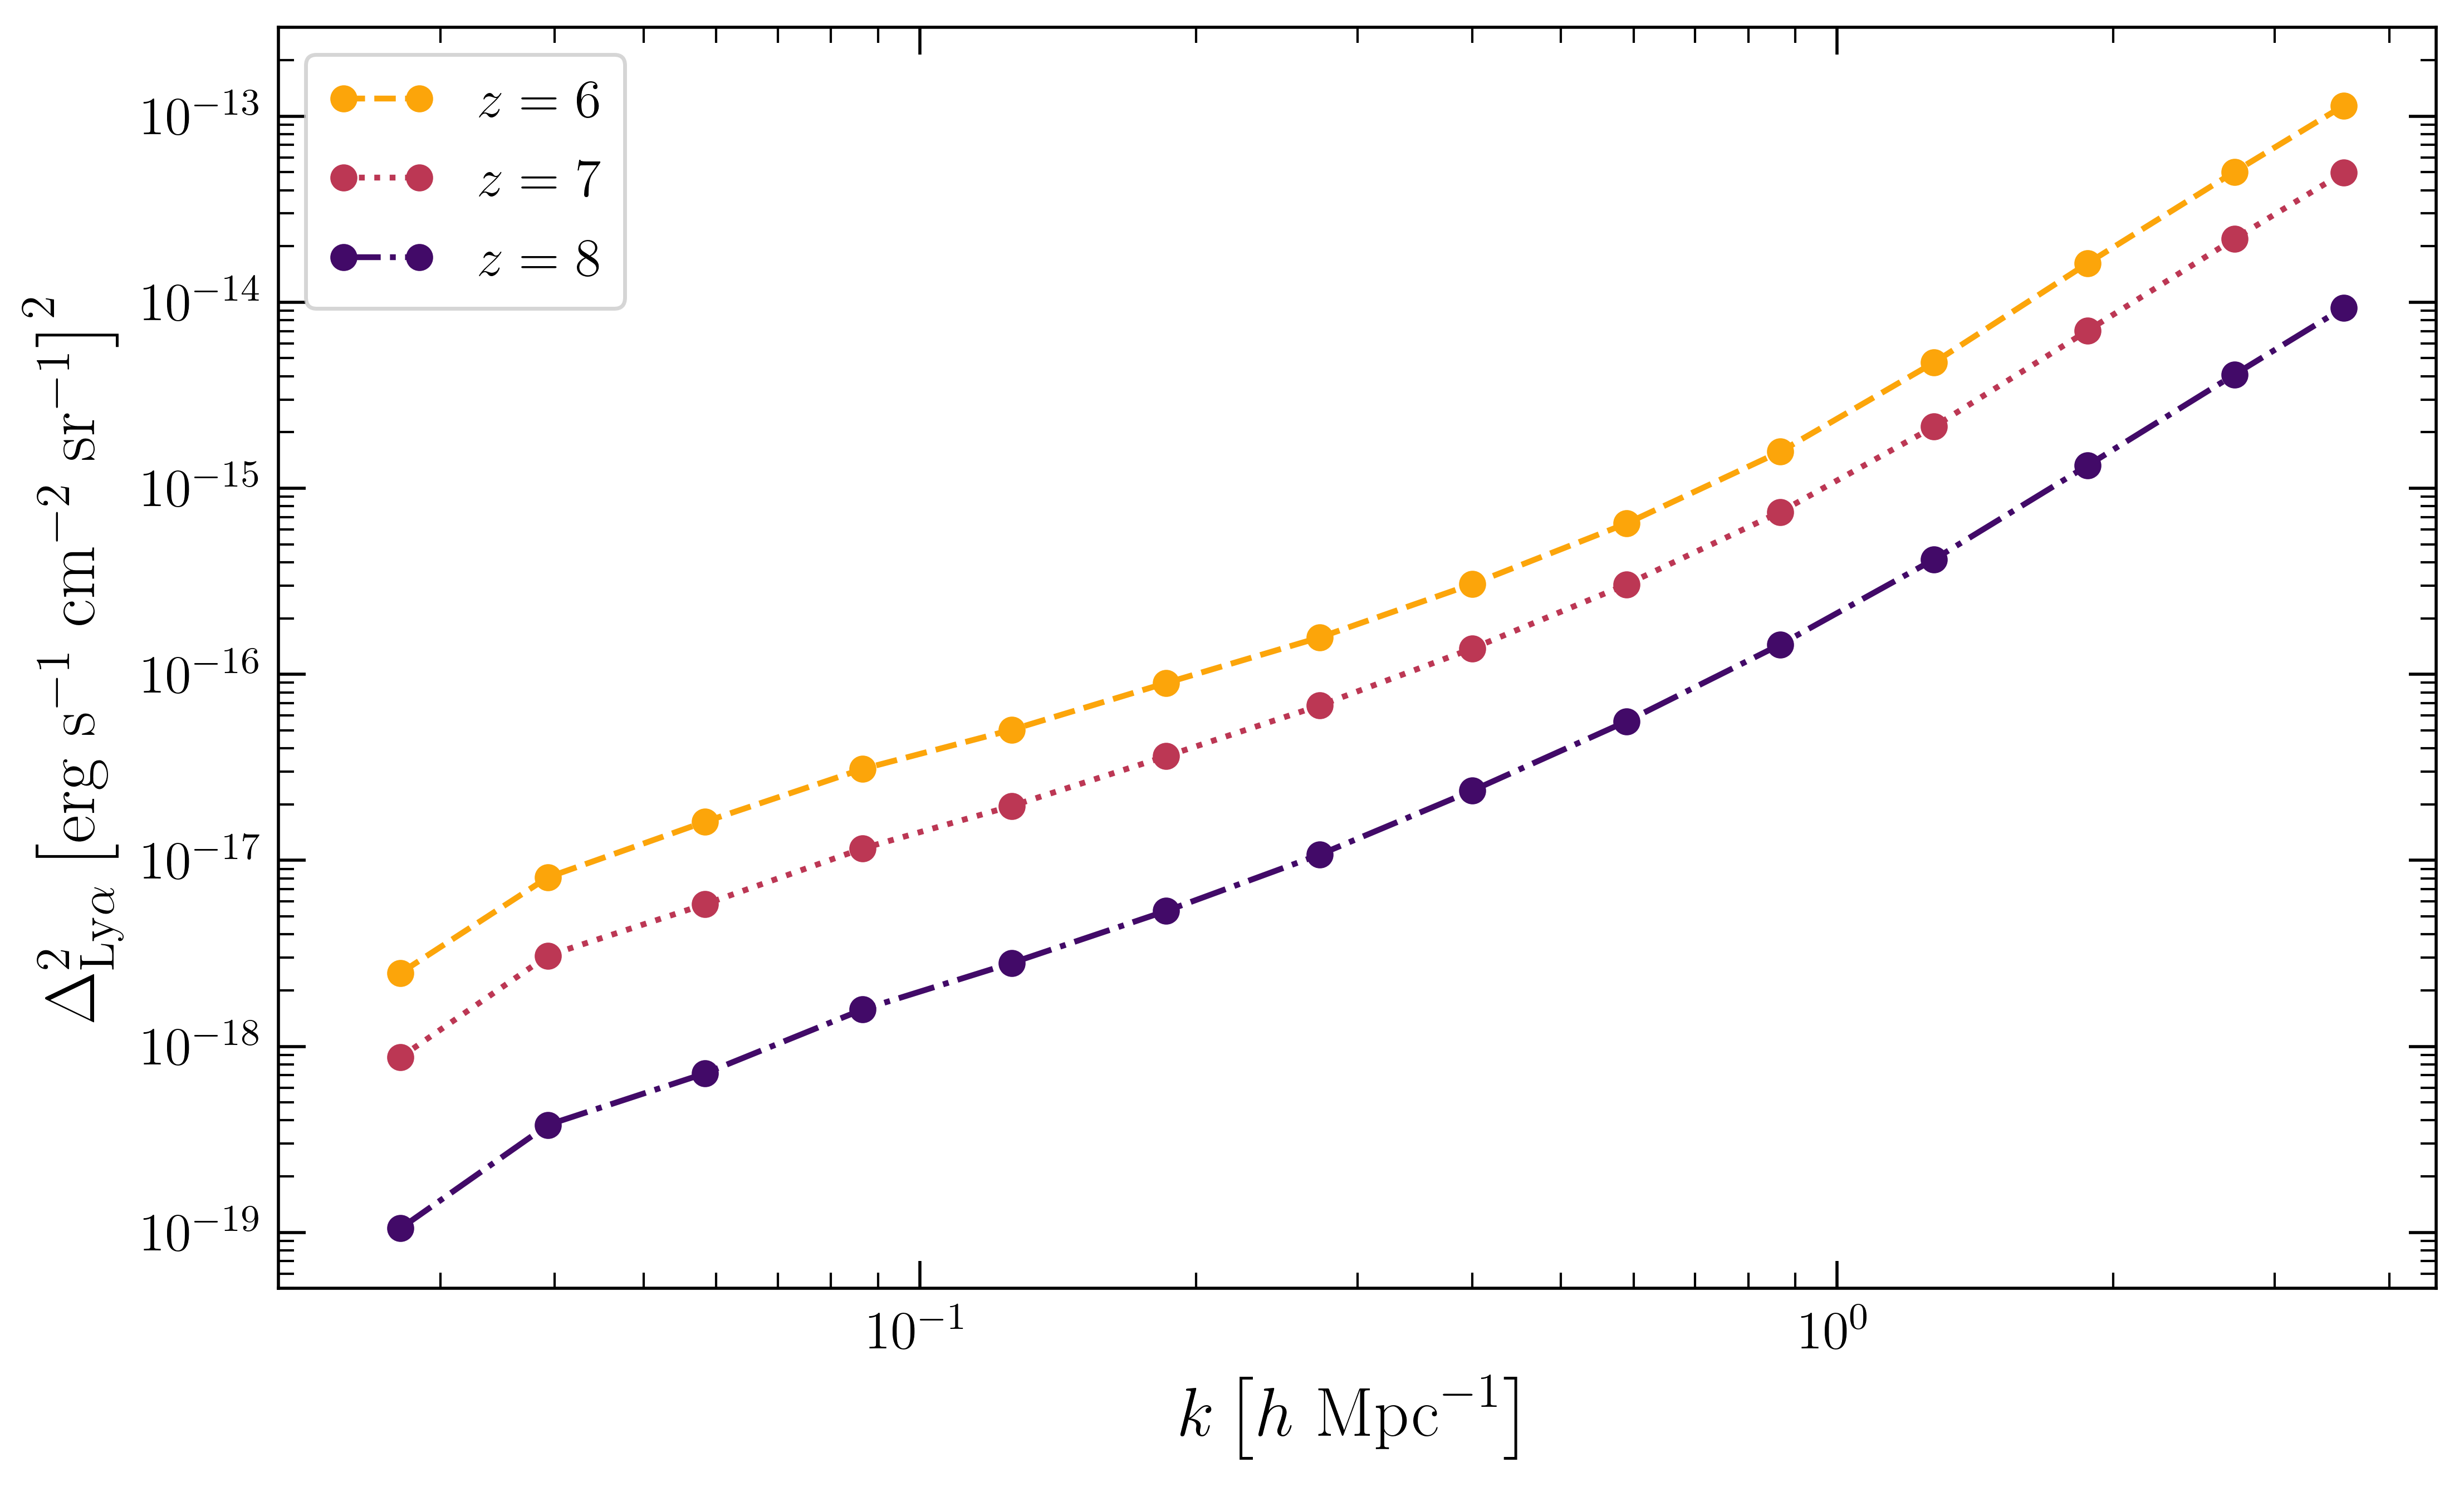
\includegraphics[width=1.\textwidth]{lyman_alpha_pspec.png}
	\caption[\lya\ Power Spectrum]{\lya\ power spectra plotted for the redshift range of interest. Here, we include
           the \lya\ contributions from both LAE's and the ionized IGM.}
	\label{fig:lya_ps}
\end{figure}

\begin{figure}[ht]
	\centering
	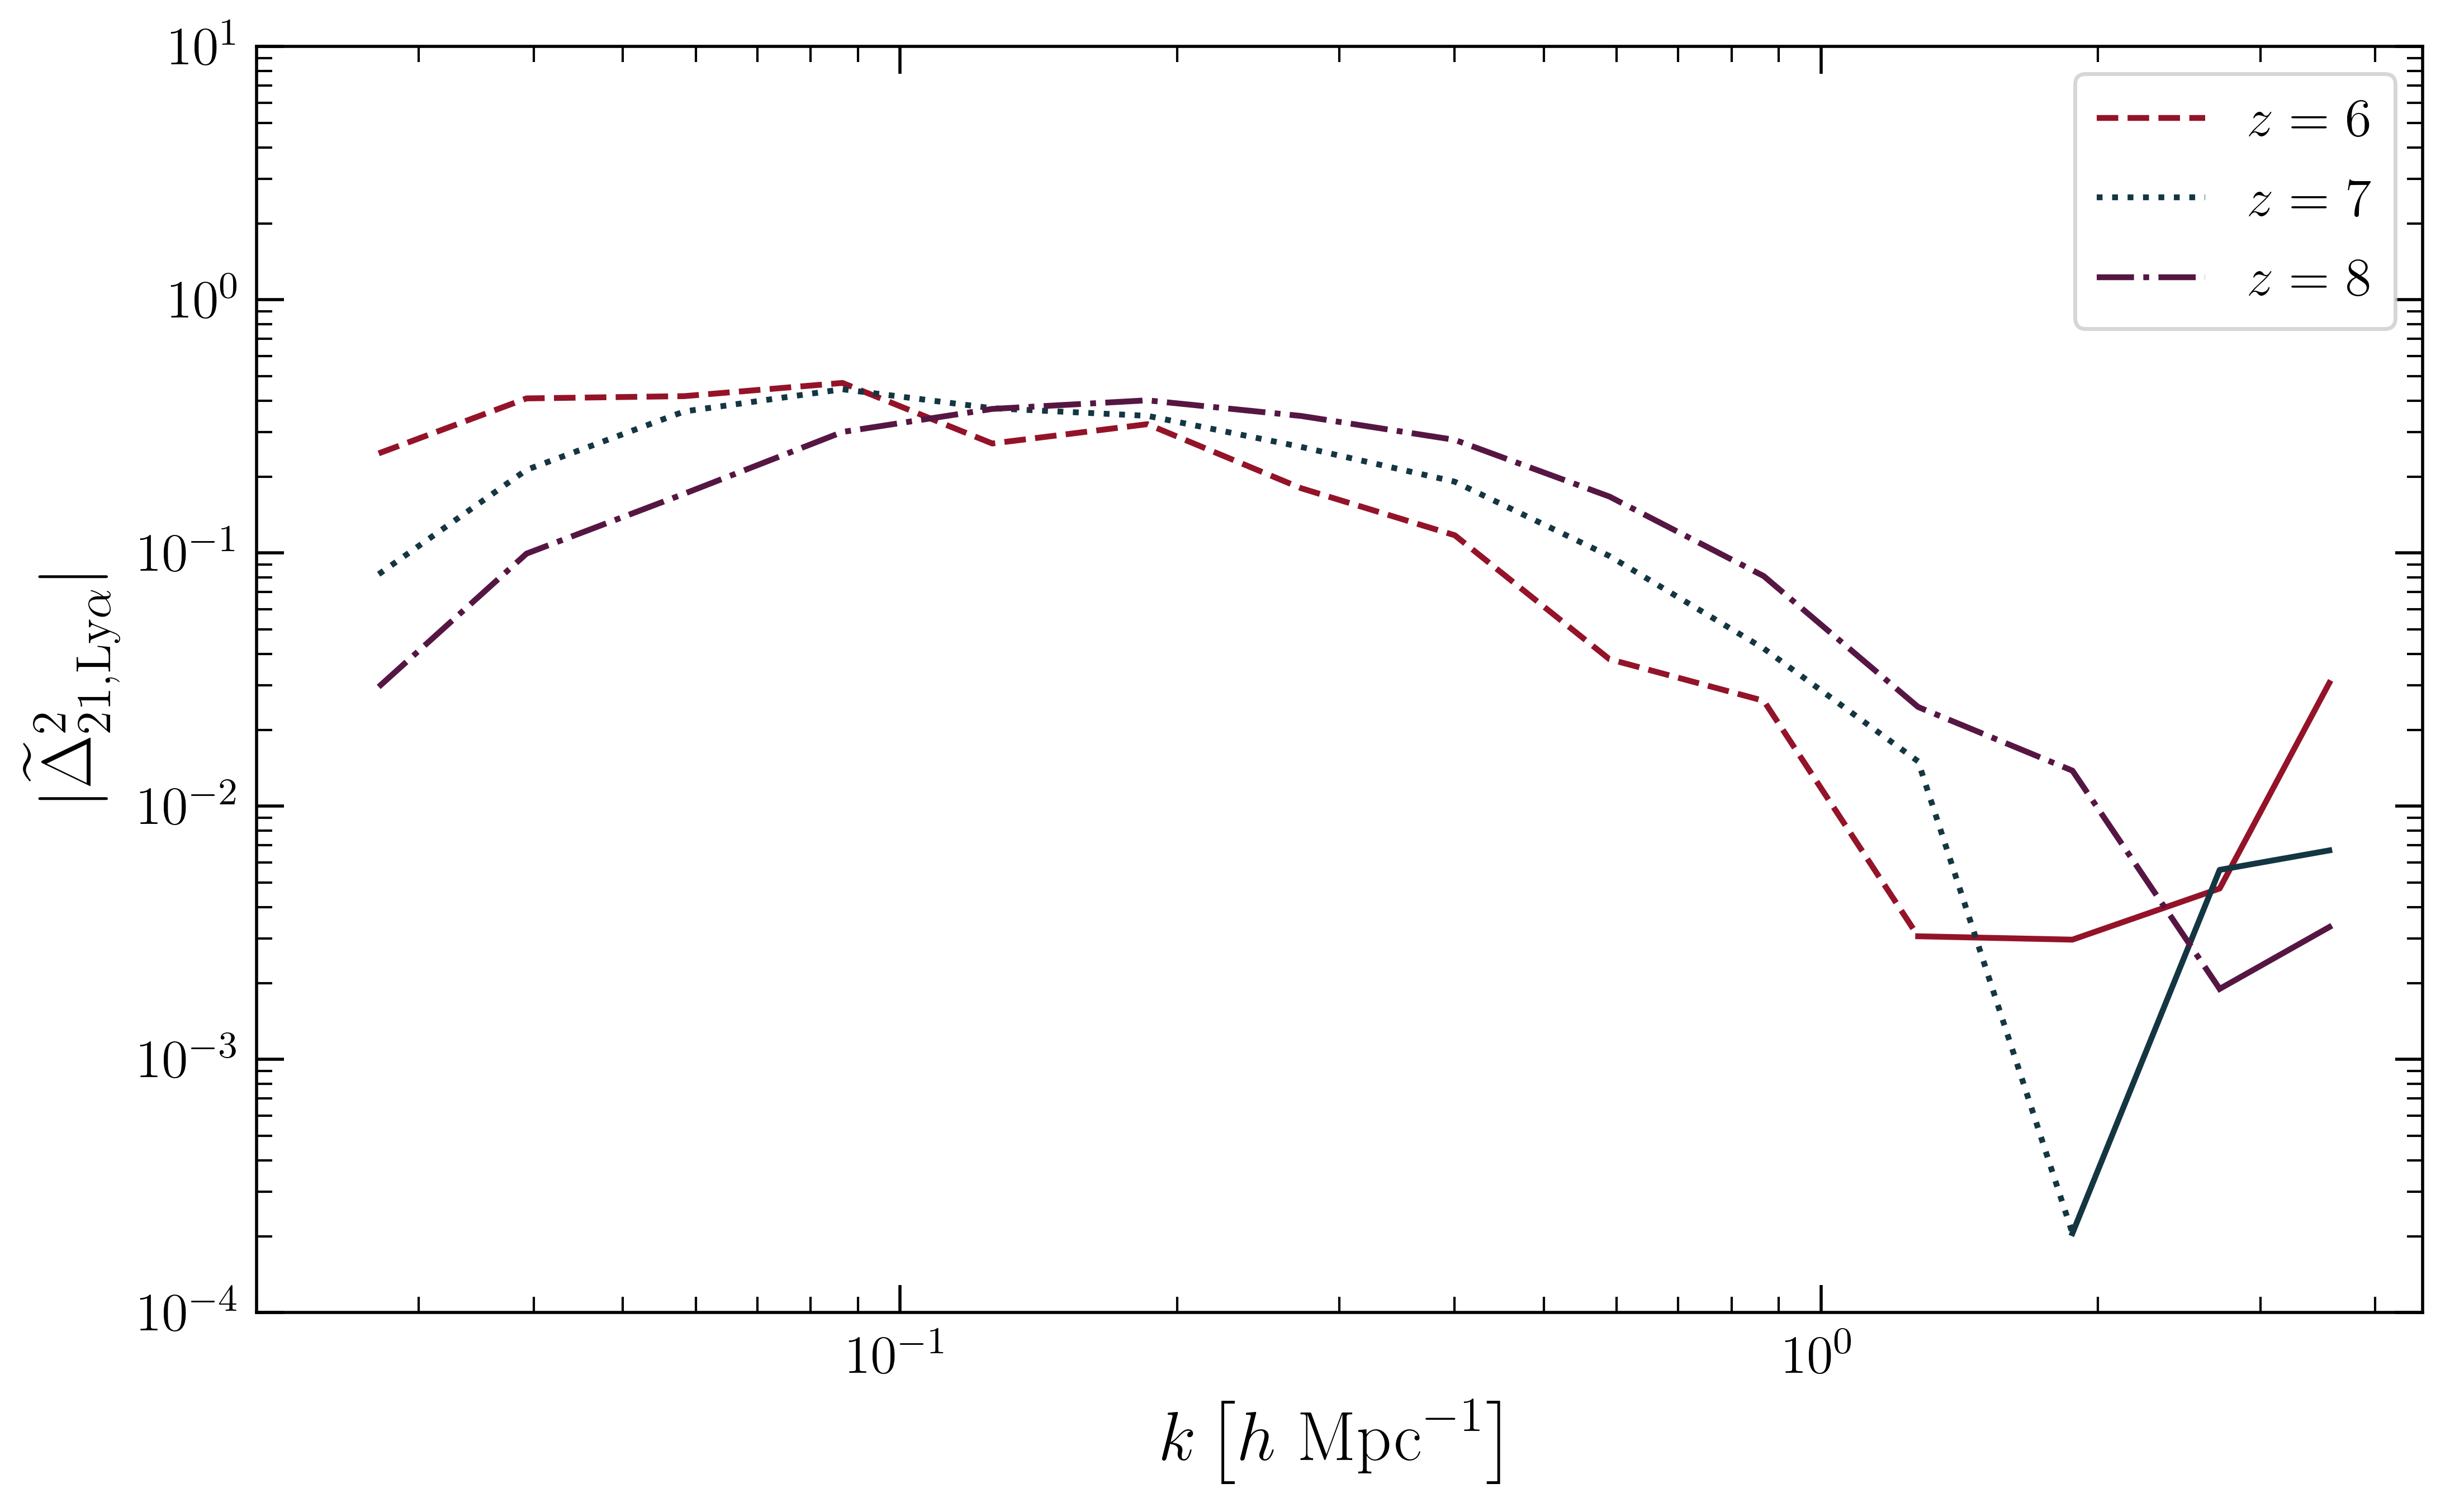
\includegraphics[width=1.\textwidth]{cross_power_spec.png}
	\caption[21\,cm-\lya\ Cross-Power Spectrum]{The dimensionless 21\,cm-\lya\ cross-power spectrum. The
           solid lines on each of the curves represent positive values in the cross-power spectrum, while varying line
           styles on the same curves represent negative values. As expected, the cross-power spectrum turns over from
           positive to negative on the scale of the mean ionized bubble size at that redshift. We also find the cross-power
           spectrum turns over at increasing scales as reionization progresses, tracing the growth of ionized bubbles.}
	\label{fig:x_ps}
\end{figure}

\begin{figure}[ht]
	\centering
	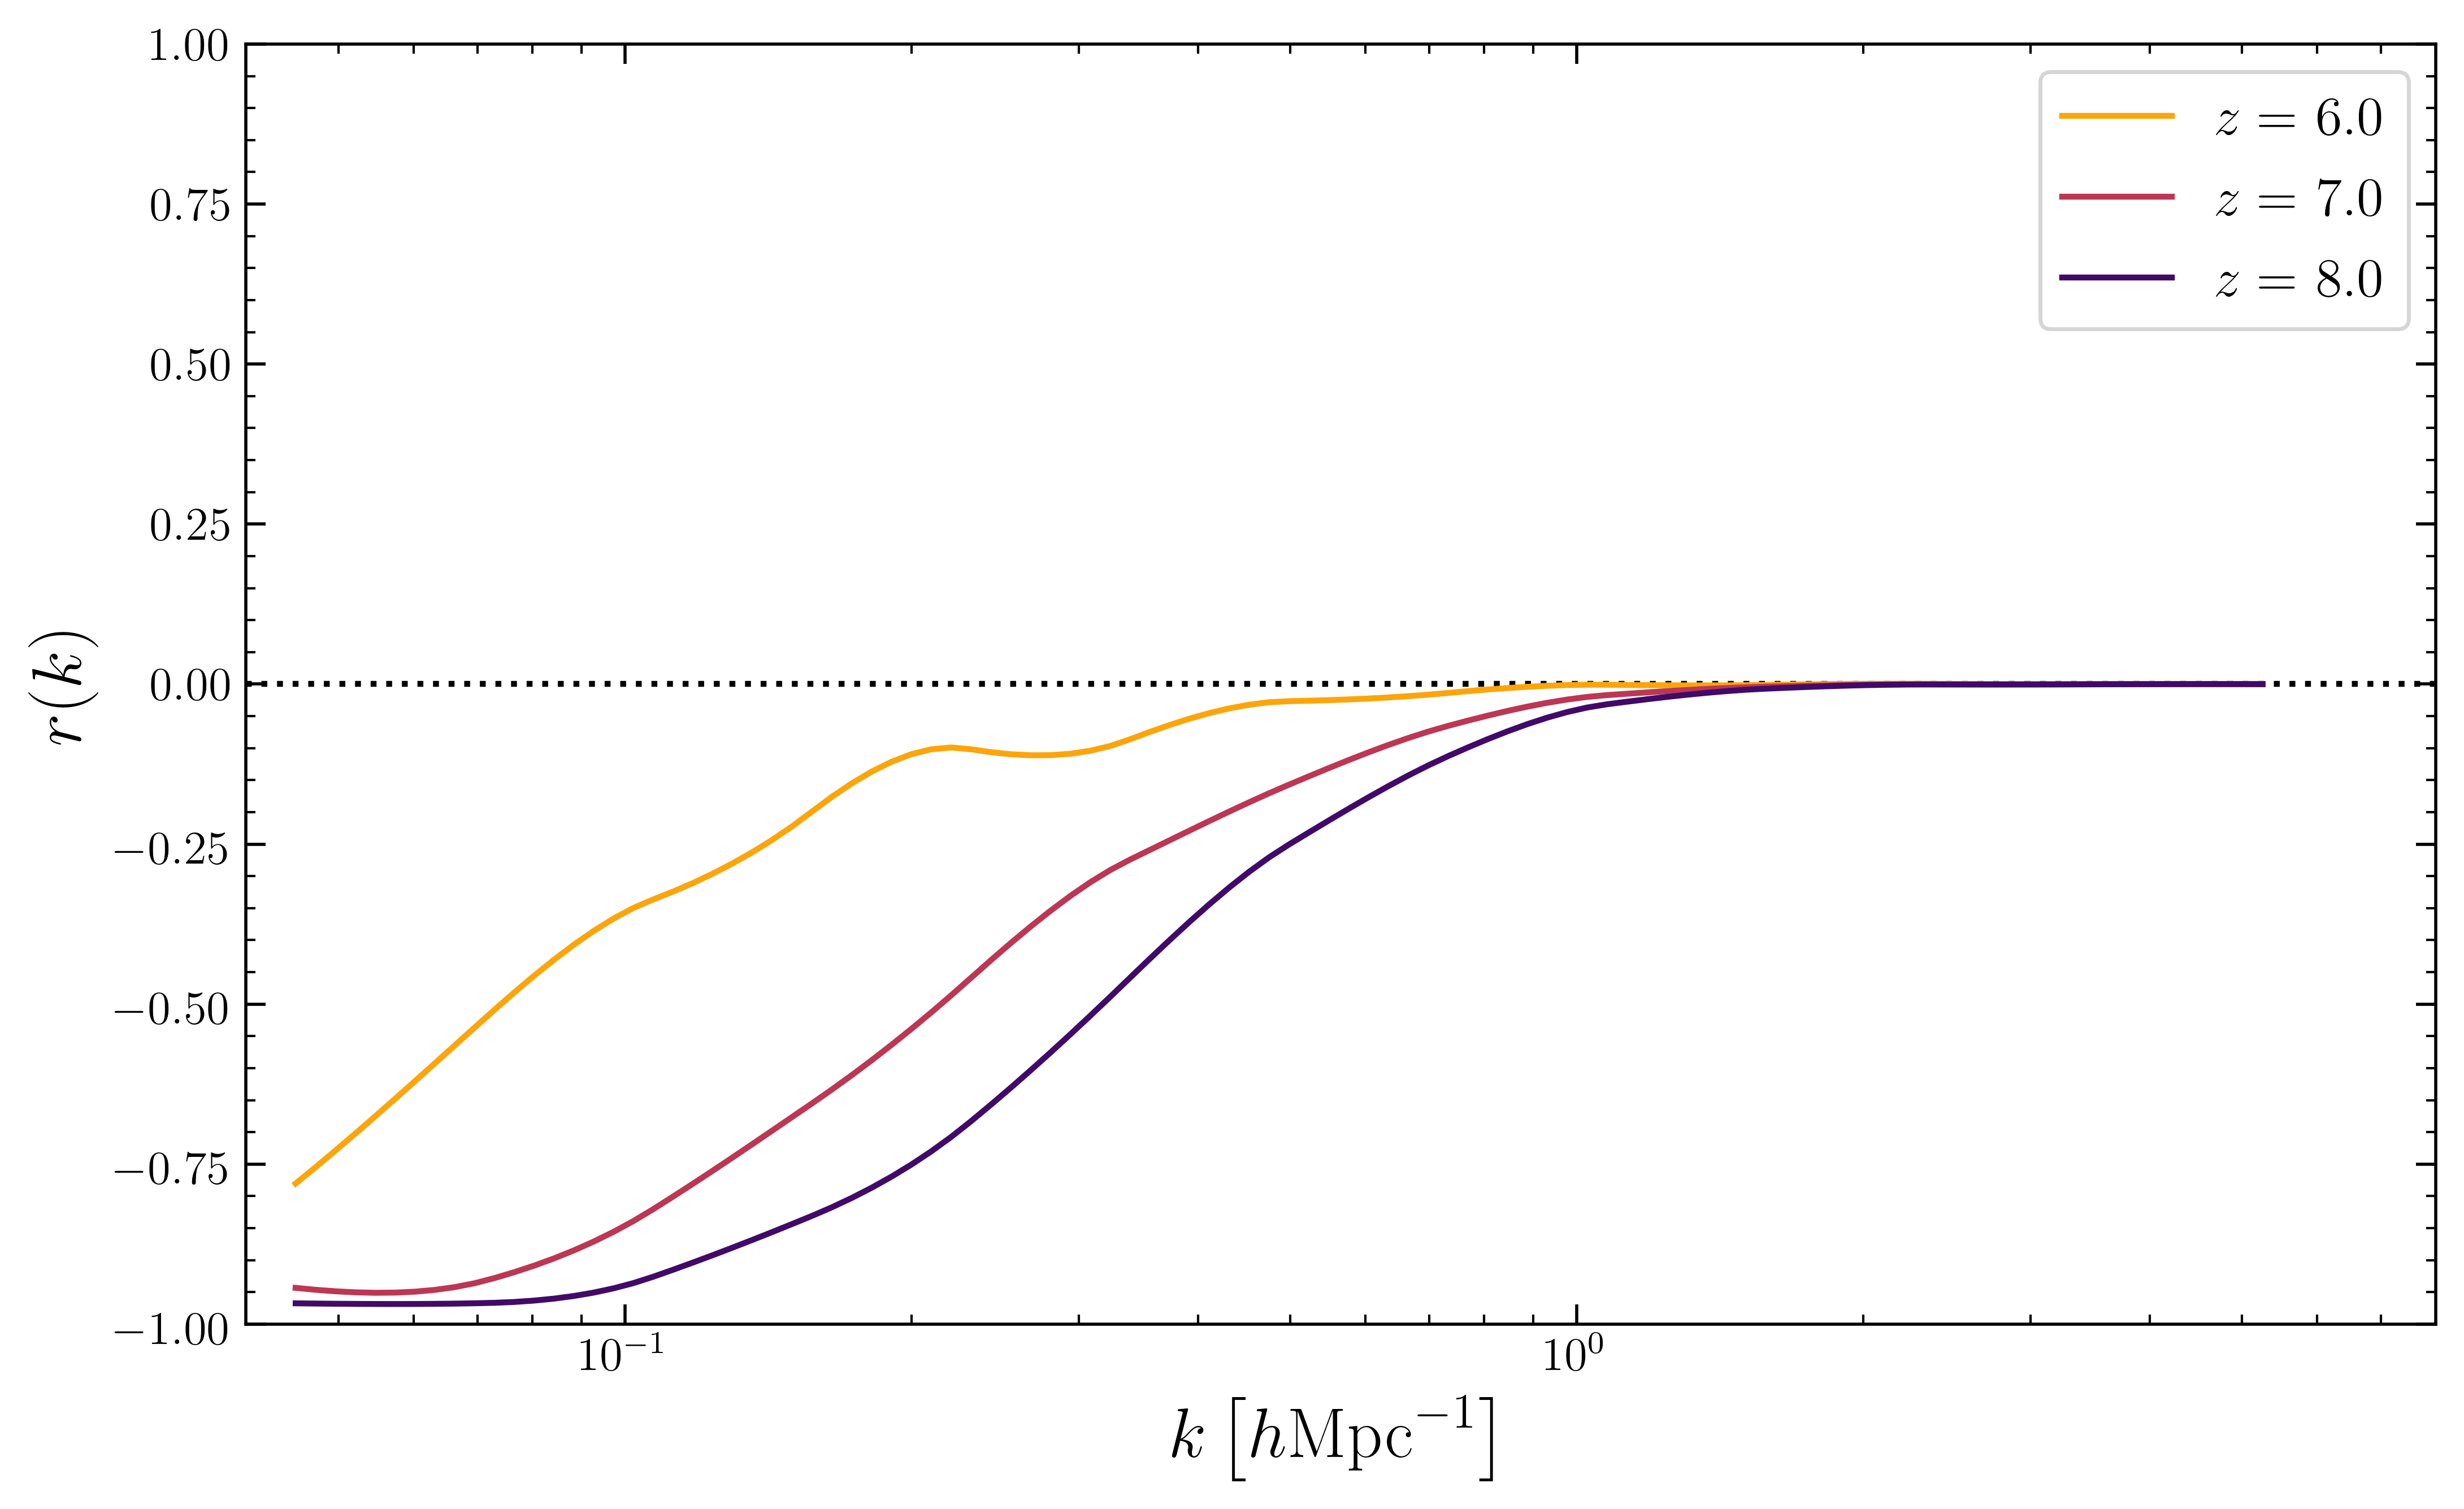
\includegraphics[width=1.\textwidth]{ccc_plot.png}
	\caption[Cross-Correlation Coefficient]{The cross-correlation coefficient plotted as a function of scale. }
	\label{fig:ccc}
\end{figure}
